%%%%%%%%%%%%%%%%%%%%%%%%%%%%%%%%%%%%%%%%%
% Template ini dibuat untuk makalah kolokium mahasiswa
% Program Alih Jenis (Ekstensi) Ilmu Komputer IPB
% Version 1.0 (18/05/2015)
%
% Template ini menggunakan template yang di-download dari:
% http://www.LaTeXTemplates.com
% Mathias Legrand (legrand.mathias@gmail.com)
% License: CC BY-NC-SA 3.0 (http://creativecommons.org/licenses/by-nc-sa/3.0/)
%
% Dimodifikasi untuk keperluan Program Studi
% Oleh: JULIO ADISANTOSO (julioipb@gmail.com)
%
% Untuk memudahkan penggunaan, maka diambil contoh makalah atas nama 
% Fithranto Faturakhman di bawah bimbingan Karlisa Priandana ILKOM-IPB.
% Silakan mengganti dan melengkapi file:
%    (1) kolokium_information.tex -- judul, nama, nim, email, pembimbing, dsb
%    (2) abstrak.tex -- abstrak makalah
%    (3) pendahuluan.tex -- berisi latar belakang, dsb
%    (4) metode.tex -- berisi metode penelitian
%    (5) pustaka.bib -- berisi daftar pustaka
%
%%%%%%%%%%%%%%%%%%%%%%%%%%%%%%%%%%%%%%%%%

%----------------------------------------------------------------------------------------
%	PACKAGES AND OTHER DOCUMENT CONFIGURATIONS
%----------------------------------------------------------------------------------------

\documentclass[fleqn,11pt]{SelfArx} % Document font size and equations flushed left
%\usepackage[english]{babel}

%----------------------------------------------------------------------------------------
%	COLUMNS
%----------------------------------------------------------------------------------------

\setlength{\columnsep}{0.55cm} % Distance between the two columns of text
\setlength{\fboxrule}{0.75pt} % Width of the border around the abstract

%----------------------------------------------------------------------------------------
%	COLORS
%----------------------------------------------------------------------------------------

\definecolor{color1}{RGB}{0,0,90} % Color of the article title and sections
\definecolor{color2}{RGB}{0,20,20} % Color of the boxes behind the abstract and headings

%----------------------------------------------------------------------------------------
%	HYPERLINKS
%----------------------------------------------------------------------------------------

\usepackage{hyperref} % Required for hyperlinks
\hypersetup{hidelinks,colorlinks,breaklinks=true,urlcolor=color2,citecolor=color1,linkcolor=color1,bookmarksopen=false,pdftitle={Title},pdfauthor={Author}}


%
% Hyphenation untuk Indonesia 
%
% @author  Andreas Febrian
% @version 1.00
% 
% Tambahkan cara pemenggalan kata-kata yang salah dipenggal secara otomatis 
% oleh LaTeX. Jika kata tersebut dapat dipenggal dengan benar, maka tidak 
% perlu ditambahkan dalam berkas ini. Tanda pemenggalan kata menggunakan 
% tanda '-'; contoh: menarik  --> pemenggalan: me-na-rik
%

\hyphenation{
    % alphabhet A
    a-na-li-sa a-tur 
    a-pli-ka-si 
    % alphabhet B
    ba-ngun-an 
    be-be-ra-pa 
    ber-ge-rak
    ber-ke-lan-jut-an 
    ber-pe-nga-ruh 
    Bha-dri-ra-ju
    % alphabhet C
    ca-ri
    % alphabhet D
    di-sim-pan di-pim-pin de-ngan da-e-rah di-ba-ngun da-pat di-nya-ta-kan 
    di-sim-bol-kan di-pi-lih di-li-hat de-fi-ni-si
    % alphabhet E
    e-ner-gi eks-klu-sif
    % alphabhet F
    fa-si-li-tas
    % alphabhet G
    graph-viz
    ga-bung-an ge-rak
    % alphabhet H
    ha-lang-an
    % alphabhet I
    % alphabhet J
    jang-krik
    % alphabhet K
    ke-hi-lang-an
    ku-ning 
    kua-li-tas ka-me-ra ke-mung-kin-an ke-se-pa-ham-an
    % alphabhet L
    ling-kung-an
    % alphabhet M
    me-ma-kan
    me-neng-ah
    meng-hubung-kan
    meng-a-tas-i me-mung-kin-kan me-nge-na-i me-ngi-rim-kan 
    meng-u-bah meng-a-dap-ta-si me-nya-ta-kan mo-di-fi-ka-si
    meng-a-tur meng-um-pul-kan Men-te-ri
    me-ngabai-kan
    Mo-ham-med
    % alphabhet N
    nya-ta non-eks-klu-sif
    % alphabhet O
    % alphabhet P
    pe-rang-kat
	pe-nye-rap-an 
	pe-ngon-trol
    pe-mo-del-an
    pe-ran  pe-ran-an-nya
    pem-ba-ngun-an pre-si-den pe-me-rin-tah prio-ri-tas peng-am-bil-an 
    peng-ga-bung-an pe-nga-was-an pe-ngem-bang-an 
    pe-nga-ruh pa-ra-lel-is-me per-hi-tung-an per-ma-sa-lah-an 
    pen-ca-ri-an peng-struk-tur-an
    PER-TAM-BANG-AN
    pe-rang-kat
    perang-kat
    % alphabhet Q
    % alphabhet R
    ran-cang-an
    % alphabhet S
    si-mu-la-si sa-ngat Sa-ma-rin-da
    % alphabhet T
    te-ngah
    ter-da-pat
    % alphabhet U
    % alphabhet V
    % alphabhet W
    % alphabhet X
    % alphabhet Y
    % alphabhet Z
    % special
    wak-tu
}
% Tuliskan nama lengkap Anda
\def\namaMhs {Alin Nur Alifah}

% Tuliskan NIM Anda
\def\nim {G64154068}

% Tuliskan alamat email Anda
\def\emailMhs {alinnural@apps.ipb.ac.id}

% Tuliskan nama lengkap dosen pembimbing
\def\namaDosen {Irman Hermadi, Idat Galih Permana}

% Tuliskan judul makalah kolokium di definisi "judul"
\def\judul {Pengembangan Sistem Formulasi Ransum untuk Kebutuhan Ternak Ruminansia Menggunakan \textit{Linier Programming}}

% Tuliskan kata kunci, dipisahkan oleh tanda titik-koma
\def\katakunci {formulasi ransum; perograman linier; prototipe, ternak ruminansia, \\feed formulation, linier programming, prototype, ruminanted livestock}

\usepackage{xcolor,colortbl}
\usepackage{multicol}
\usepackage{multirow}
\usepackage{graphicx,xcolor}
\graphicspath{{gambar/}}

%\usepackage[urldate=iso8601, backend=biber, style=authoryear, url=true, doi=true, sorting=nyt]{biblatex}
\usepackage[urldate=comp, backend=biber, style=authoryear, url=true, doi=true, maxbibnames=4, maxcitenames=2, block=none, sorting=nyt]{biblatex}
\usepackage{xpatch}
\addbibresource{pustaka.bib}
\DefineBibliographyStrings{english}{%
	and = {dan}
}
\DefineBibliographyStrings{english}{%
	andothers = {\em et\addabbrvspace al\adddot}
}
\renewbibmacro{in:}{
	\iffieldundef{journaltitle}
	{}
	{\xspace dalam:}
}
\renewbibmacro*{volume+number+eid}{%
	\printfield{volume}%
	%  \setunit*{\adddot}% DELETED
	\setunit*{\addnbspace}% NEW (optional); there's also \addnbthinspace
	\printfield{number}%
	\setunit{\addcomma\space}%
	\printfield{eid}}
\DeclareFieldFormat[article]{number}{\mkbibparens{#1}}
\DeclareFieldFormat{url}{\printtext{Dapat diunduh dari}\addcolon\space\url{#1}}
%\DeclareFieldFormat{urldate}{#1}
\DeclareFieldFormat{urldate}{%
	\thefield{urlday}\addslash%
	\thefield{urlmonth}\addslash%
	\thefield{urlyear}\isdot}

\DeclareNameAlias{sortname}{last-first}
\DeclareNameAlias{default}{last-first}
\renewbibmacro*{begentry}{%
	\ifnameundef{shortauthor}
	{}
	{[\printnames{shortauthor}%
		]\addspace}}

\renewbibmacro*{url+urldate}{%
	\iffieldundef{urlyear}
	{}
	{\setunit*{\addspace}%
		\printtext{[Internet]. [}%
		\printtext{Diunduh tanggal}\space%
		\printurldate\space
		\printtext{].}\space%
		\printfield{url}}%
}
\xpatchbibmacro{date+extrayear}{%
	\printtext[parens]%
}{%
\setunit{\addperiod\space}%
\printtext%
}{}{}
\nocite{*}


%\usepackage[urldate=iso8601, backend=biber, style=authoryear, url=true, doi=true, sorting=nyt]{biblatex}
%\addbibresource{pustaka.bib}
%\DefineBibliographyStrings{english}{%
%	urlseen = {diunduh pada},
%}
%\renewbibmacro{in:}{\xspace dalam:}
%\renewbibmacro*{volume+number+eid}{%%
%	\printfield{volume}%
%	%  \setunit*{\adddot}% DELETED
%	\setunit*{\addnbspace}% NEW (optional); there's also \addnbthinspace
%	\printfield{number}%
%	\setunit{\addcomma\space}%
%	\printfield{eid}}
%\DeclareFieldFormat[article]{number}{\mkbibparens{#1}}

%----------------------------------------------------------------------------------------
%	ARTICLE INFORMATION
%----------------------------------------------------------------------------------------

\JournalInfo{Makalah Kolokium Program S1 Ilmu Komputer Alih Jenis} % Journal information
\Archive{Departemen Ilmu Komputer, FMIPA-IPB} % Departemen ILKOM-IPB

\PaperTitle{\judul} 

\Authors{\namaMhs (\nim)*, \namaDosen} % Penulis
\affiliation{*\scriptsize\textbf{Alamat Email}: \emailMhs \normalsize} % Corresponding author

\Keywords{\scriptsize \katakunci \normalsize} 
\newcommand{\keywordname}{Kata Kunci} % Defines the keywords heading name

%----------------------------------------------------------------------------------------
%	ABSTRACT
%----------------------------------------------------------------------------------------
\Abstract{\scriptsize 
% ---- Tuliskan abstrak di bagian ini seperti contoh.
Formulasi ransum merupakan aspek yang sangat esensial dalam menyeimbangkan nutrisi bagi hewan ternak dengan tujuan mendapatkan harga minimum berdasar pada kandungan nutrisi pakan hewan. Oleh karena itu peternak dituntut untuk mampu menyusun suatu formula ransum yang ekonomis tanpa mengabaikan faktor kebutuhan nutrisi ternak. Penelitian ini bertujuan untuk membuat suatu sistem pendukung pengambilan keputusan yang mampu melakukan formulasi ransum dengan mengadopsi metode \textit{linier programming}. Metode pengembangan sistem yang dilakukan adalah \textit{prototype} dengan evaluasi menggunakan perbandingan dengan aplikasi WinFeed dan POM QM.
\\
\\
Feed formulation is an essential aspect in balancing nutrients for livestock in order to get a minimum price based on the nutrient content of livestock feed. Therefore, farmers are required to be able to compile an economical feed formulation without ignoring nutritional needs factors of livestock. This research aims to create/develop a decision support system that is capable of compile feed formulation by adopting the method of linear programming. The development method used is prototype with evaluation using comparation beetwen WinFeed application and POM QM.
% ---- Akhir bagian abstrak
\normalsize}


%----------------------------------------------------------------------------------------

\begin{document}

\flushbottom % Makes all text pages the same height

\maketitle % Print the title and abstract box

\thispagestyle{empty} % Removes page numbering from the first page

%----------------------------------------------------------------------------------------
%	BAGIAN PENDAHULUAN
%----------------------------------------------------------------------------------------

%----------------------------------------------------------------------------------------
%	PENDAHULUAN
%----------------------------------------------------------------------------------------
\section*{PENDAHULUAN} % Sub Judul PENDAHULUAN
% Tuliskan isi Pendahuluan di bagian bawah ini. 
% Jika ingin menambahkan Sub-Sub Judul lainnya, silakan melihat contoh yang ada.
% Sub-sub Judul 
\subsection*{Latar Belakang}
Pengujian adalah serangkaian proses yang dirancang untuk memastikan sebuah perangkat lunak melakukan apa yang seharusnya dilakukan. Proses ini bertujuan untuk menemukan kesalahan pada perangkat lunak. Saat pengujian, bisa saja tidak ditemukan kesalahan pada hasil pengujian. Hal ini dapat terjadi karena perangkat lunak yang sudah berkualitas tinggi atau karena proses pengujiannya berkualitas rendah. (\cite{GLENFORD2012})

Teknik pengujian secara umum dibagi menjadi 2 kategori diantaranya \textit{black box testing} dan \textit{white box testing}. \textit{Black box testing} bertujuan untuk memeriksa fungsional dari perangkat lunak apakah output sudah sesuai dengan yang ditentukan. Sedangkan \textit{white box testing} atau biasa disebut dengan pengujian struktural merupakan pemeriksaan struktur dan alur logika suatu proses. \textit{Basis path testing} merupakan salah satu metode pengujian struktural yang menggunakan kode program untuk menemukan semua jalur yang mungkin dapat dilalui program dan dapat digunakan untuk merancang data uji. Metode ini memastikan semua kemungkinan jalur dijalankan setidaknya satu kali (\cite{BASU2015}). Untuk melakukan monitoring jalur mana yang diambil oleh sebuah masukan pada saat eksekusi program, maka diperlukan penanda yang dapat memberikan informasi cabang mana yang dilalui. Proses menyisipkan tanda tersebut disebut instrumentasi. Biasanya tanda tersebut disisipkan tepat sebelum atau sesudah sebuah percabangan (\cite{TIKIR2011}). 

Idealnya, pengujian dilakukan untuk semua kemungkinan dari perangkat lunak. Tetapi untuk menguji perangkat lunak yang kompleks secara keseluruhan akan memakan waktu yang lama dan membutuhkan sumber daya manusia yang banyak. \citeauthor{KUMAR20168} (\cite*{KUMAR20168}) mengatakan bahwa pengujian perangkat lunak menggunakan hampir 60\% dari total biaya pengembangan perangkat lunak. Jika proses pengujian perangkat lunak dapat dilakukan secara otomatis, maka hal ini dapat mengurangi biaya pengembangan secara signifikan. 

\citeauthor{HERMADI2015} (\cite*{HERMADI2015}) melakukan penelitian membangkitkan data uji untuk \textit{path testing} menggunakan algoritma genetika. Dalam penelitian tersebut, \citeauthor{HERMADI2015} membangkitkan \textit{Control Flow Graph} (CFG) dan instrumentasi masih secara manual sehingga membutuhkan banyak waktu dan rawan akan kesalahan ketika program sudah semakin besar. Sehingga mengotomasi hal tersebut dapat membuat \textit{path testing} menjadi lebih cepat dan dapat mengurangi kerawanan akan kesalahan.

Pada penelitian ini, akan dibangun sebuah perangkat lunak untuk membangkitkan kemungkinan jalur dari sebuah program. Jalur-jalur ini dapat dijadikan dasar untuk membangkitkan data uji agar data uji yang digunakan untuk pengujian dapat mewakili semua kemungkinan. Untuk memonitor jalur mana yang dilalui ketika diberikan masukan data uji, maka sistem ini juga akan melakukan penyisipan tag-tag sebagai instrumentasi ke dalam kode program secara otomatis.

% Sub-sub Judul 
\subsection*{Perumusan Masalah}
Berdasarkan latar belakang di atas dapat dirumuskan masalahnya adalah bagaimana membangun sebuah aplikasi untuk melakukan instrumentasi secara otomatis untuk pengujian jalur dan dapat dimanfaatkan untuk \textit{re-engineering} perangkat lunak.

\subsection*{Tujuan}
Penelitian ini bertujuan untuk membangun sebuah aplikasi yang dapat digunakan untuk membangkitkan CFG dan melakukan instrumentasi secara otomatis.

\subsection*{Ruang Lingkup}
Bahasa pemrograman yang diakomodasi adalah Matlab dan model diagram yang dibangkitkan adalah CFG.

\subsection*{Manfaat}
Hasil penelitian diharapkan dapat membantu pengembang dan penguji aplikasi untuk:
\begin{enumerate}[noitemsep] 
\item Menyisipkan tag-tag sebagai instrumentasi program ke dalam kode program secara otomatis sehingga proses tersebut dapat dilakukan dengan lebih cepat.
\item Membangkitkan jalur-jalur dasar yang dapat digunakan sebagai dasar untuk pembangkitan data uji.
\item Membangkitkan diagram CFG yang dapat memudahkan pengembang dalam memahami struktur dan alur dari suatu program yang dapat dimanfaatkan ketika akan melakukan \textit{re-engineering} perangkat lunak.
\end{enumerate}


%----------------------------------------------------------------------------------------
%	BAGIAN METODE
%----------------------------------------------------------------------------------------

%----------------------------------------------------------------------------------------
%	METODE
%----------------------------------------------------------------------------------------
\section*{METODE PENELITIAN}

Penelitian yang dilakukan terbagi menjadi beberapa tahapan proses. Gambar \ref{fig:metodepenelitian} menunjukan tahapan proses tersebut.

\begin{figure}[h!]
	\centering
	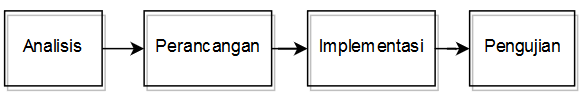
\includegraphics[width=220pt]{gambar/metode_penelitian}
	\caption{Metode Penelitian}
	\label{fig:metodepenelitian}
\end{figure}

\subsection*{Analisis}

Pada tahap ini dimulai dari membaca literatur terkait dan mendefinisikan kebutuhan dari aplikasi yang akan dibangun. Selain itu, pada tahapan ini juga dilakukan pengumpulan berapa contoh program yang akan digunakan dalam penelitian. Contoh program yang digunakan dalam penelitian ini didapatkan dari penelitian yang dilakukan oleh \citeauthor{HERMADI2015} (\cite*{HERMADI2015}).  

\subsection*{Perancangan}
Pada tahap ini ditentukan bagaimana perangkat lunak akan dibangun. Ilustrasi arsitektur sistem dapat dilihat pada Gambar \ref{fig:struktur}.
\begin{figure}[h!]
	\centering
	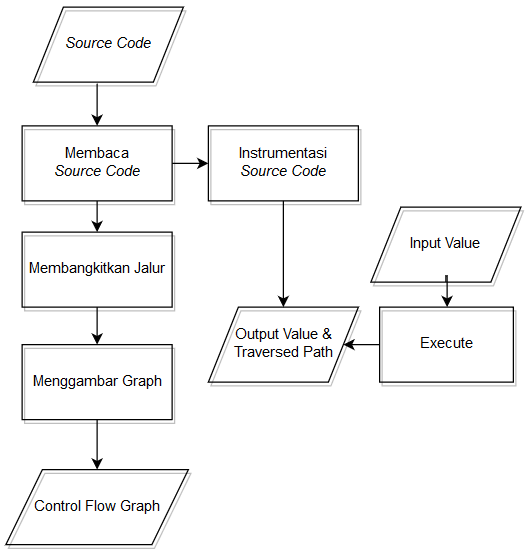
\includegraphics[width=230pt]{gambar/struktur}
	\caption{Arsitektur Sistem}
	\label{fig:struktur}
\end{figure}

\subsubsection*{Kode Program}
Kode program matlab akan dibaca sebagai inputan. Matlab merupakan singkatan dari MATrix LABoratory. Seperti bahasa pemrograman lainnya, matlab memiliki beberapa sruktur kontrol. Struktur kontrol adalah perintah dalam bahasa pemrograman yang digunakan dalam pengambilan keputusan. Matlab memiliki empat struktur kontrol, yaitu IF-ELSE-END, SWITCH-CASE, FOR, dan WHILE (\cite{HOUCQUE2005}). 

\subsubsection*{Mengurai Kode Progam ke Format XML}
Penguraian kode program matlab dilakukan dengan menggunakan library  MATLAB-PARSER. Ketika terdapat kesalahan pada kode program, library  ini akan mengembalikan pesan \textit{error}. Lalu kode program tersebut diurai menjadi file dengan format XML menggunakan \textit{library} MATLAB-PARSER yang dibuat oleh  \citeauthor{SUFFOSPARSER2005} (\cite*{SUFFOSPARSER2005}). 

\textit{Extensible Markup Language} (XML) adalah bahasa yang dapat mendeskripsikan sebuah dokumen. XML memiliki banyak bagian yang tidak memiliki struktur yang pasti. XML terdiri atas dua bagian utama, yaitu elemen dan atribut. Elemen yang dapat disebut sebagai \textit{node} merupakan bagian penting yang dapat menggambarkan struktur dari XML. Sedangkan atribut merupakan bagian yang dapat digunakan sebegai informasi tambahan dari setiap elemen  (\cite{HARTWELL2017}). 

\subsubsection*{Membangkitkan \textit{Graph}}
Setiap elemen dalam file XML tersebut akan ditelusuri satu persatu yang termasuk struktur kontrol di dalam bahasa matlab. Sehingga terbentuklah sebuah objek \textit{graph} yang terdiri dari sekumpulan \textit{node} dan \textit{edge}. 

Salah satu cara untuk membaca dan menulis dokumen XML pada \textit{framework} .NET dan C\# yaitu dengan menggunakan kelas XMLDocument yang terdapat dalam\textit{ namespace System.XML}. Setiap elemen XML yang merupakan struktur kontrol pada program akan menjadi \textit{node} baru di dalam kelas \textit{graph}. Setiap \textit{node} berisi informasi nomor baris dan kolom yang akan digunakan untuk melakukan instrumentasi.

\subsubsection*{Membangkitkan Jalur}
\textit{Basis path testing} merupakan salah satu metode pengujian struktural yang menggunakan \textit{source code} dari program untuk menemukan semua jalur yang mungkin dapat dilalui program dan dapat digunakan untuk merancang data uji. Metode ini memastikan semua kemungkinan jalur dijalankan setidaknya satu kali (\cite{BASU2015}). 

Metode ini terbagi menjadi 4 tahapan, yaitu:
\begin{enumerate}[noitemsep] 
	\item Menggambarkan jalur dalam bentuk \textit{ Control Flow Graph} (CFG)
	\item Menghitung \textit{cyclomatic complexity}
	\item Memilih satu set jalur dasar
	\item Membangkitkan data uji untuk setiap jalur dasar
\end{enumerate}


\subsubsection*{Transformasi ke Dalam Format Bahasa Dot}
\textit{Graph} yang sudah terbentuk akan ditransformasikan ke dalam bentuk format bahasa permrograman dot. Bahasa dot adalah bahasa yang digunakan untuk mengambar \textit{graph} berarah. Bahasa ini dapat mendeskripsikan 3 macam objek, yaitu \textit{graph}, \textit{nodes}, dan \textit{edges} (\cite{GANSNER2015}).

\subsubsection*{Memvisualisasi \textit{Graph} dalam bentuk CFG}
\textit{Control Flow Graph }(CFG) adalah graph berarah yang merepresentasikan aliran dari sebuah program. Setiap CFG terdiri dari \textit{nodes} dan \textit{edges}. \textit{Nodes} merepresentasikan \textit{statement} atau \textit{expressions}. Sedangkan \textit{edges} merepresentasikan transfer kontrol antar \textit{nodes} (\cite{MCCABE}). Notasi dari CFG dapat dilihat pada Gambar \ref{fig:cfg}.
\begin{figure}[h]
	\centering
	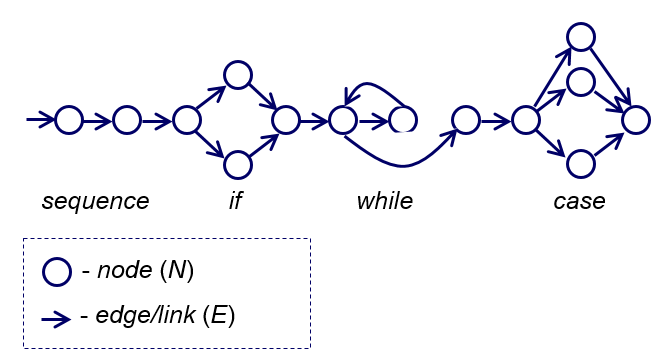
\includegraphics[width=0.9\linewidth]{gambar/CFG}
	\caption{Notasi Control Flow Graph (CFG)}
	\label{fig:cfg}
\end{figure}
Setelah file dengan format bahasa dot terbentuk, CFG akan divisualisasikan dengan menggunakan library Graphviz. Graphviz merupakan perangkat lunak open source untuk visualisasi grafik. Graphviz memiliki banyak fitur berguna untuk menggambar diagram yang konkret karena terdapat pilihan warna, font, tata letak, jenis garis, dan bentuk (\cite{ELLSONGRAPHVIZ2003}).
\subsubsection*{Menghitung \textit{Cyclometic Complexity}}

\textit{Cyclomatic complexity} merupakan suatu sistem pengukuran yang ditemukan oleh \citeauthor{MCCABE} untuk menentukan banyaknya \textit{independent path} dan menunjukan tingkat kompleksitas dari suatu program. \textit{Independent path} adalah jalur yang melintas dalam program yang sekurang-kurangnya terdapat kondisi baru. Perhitungan \textit{Cyclomatic Complexity} dapat dilihat pada persamaan berikut:
\[V(G)=E-N+2\]

Dimana, E menunjukkan jumlah \textit{edges} dan N menunjukkan jumlah \textit{nodes}.

\subsubsection*{Instrumentasi}
Setelah jalur terbentuk, dilakukan juga proses instrumentasi. Instrumentasi merupakan sebuah proses menyisipkan sebuah penanda (tag) di awal atau di akhir setiap blok kode seperti awal setiap perintah, sebelum atau sesudah kondisi terpenuhi atau tidak. Dalam pengujian path testing, penanda ini dapat digunakan untuk memonitor jalur yang dilalui program ketika dijalankan dengan masukan data uji tertentu (\cite{IRH2014}). 

Instrumentasi dilakukan dengan cara menambahkan dulu variabel keluaran bernama \textit{traversedPath}. Variabel in digunakan untuk menyimpan informasi node mana saja yang dilalui ketika diberikan inputan dengan nilai tertentu. Lalu setiap sebelum dan sesudah \textit{node} percabangan, dilakukan penyisipan kode program berupa perintah untuk memasukkan nilai \textit{node} yang dilalui. Sehingga ketika program tersebut dijalankan, akan menghasilkan keluaran tambahan bernama \textit{traversedPath}. 

\subsection*{Implementasi}

Tahapan ini adalah melakukan implementasi dari tahap sebelumnya ke dalam bentuk aplikasi web. Aplikasi ini akan dibangun dengan menggunakan bahasa pemrograman C\# dan menggunakan IDE Microsoft Visual Studio Ultimate 2013. 

Setelah file dengan format bahasa dot terbentuk, CFG divisualisasikan dengan menggunakan \textit{library} Graphviz.Net. Graphviz.Net adalah pembungkus C\# untuk generator grafik Graphviz yang dibuat oleh \citeauthor{DIXONGRAPHVIZ2013} (\cite*{DIXONGRAPHVIZ2013}). Keluaran yang dikembalikan ketika mengeksekusi Graphviz.Net berbentuk \textit{byte} dalam \textit{array} sehingga dapat diolah kembali sesuai dengan kebutuhan. Graphviz merupakan library yang dapat digunakan untuk menvisualisasi jalur ke dalam bentuk graph berarah (\cite{GANSNER2015}). 


\subsection*{Testing}

Tahapan ini adalah melakukan evaluasi dari tahapan implementasi. Evaluasi dibagi menjadi dua bagian, yaitu uji validasi dan uji efisiensi. Uji validasi dilakukan dengan cara membandingkan hasil yang ada pada penelitian sebelumnya dengan hasil yang dikeluarkan oleh aplikasi. Pada penelitian sebelumnya, \textit{graph} yang dibangun adalah \textit{graph} yang hanya menggambarkan notasi percabangan. Agar dapat dibandingkan dengan hasil yang dikeluarkan oleh aplikasi, \textit{graph} yang ada pada penelitian sebelumnya direpresentasikan ke dalam bentuk \textit{adjacency list} terlebih dahulu secara manual.

Uji efisiensi dilakukan dengan membandingkan waktu eksekusi yang dilaukan secara manual dengan waktu eksekusi oleh aplikasi. Pengujian manual akan dilakukan dengan meminta satu atau dua orang yang sudah memiliki pengalaman dalam pemrograman sebagai sampel  untuk melihat berapa lama waktu yang dibutuhkan untuk membangkitkan CFG, membangkitkan semua kemungkinan jalur,  menghitung \textit{cyclomatic complexity}, dan melakukan instrumentasi.


%----------------------------------------------------------------------------------------
%	BAGIAN DAFTAR PUSTAKA
%----------------------------------------------------------------------------------------

\renewcommand{\refname}{DAFTAR PUSTAKA}
\nocite{*}
\printbibliography

%----------------------------------------------------------------------------------------

\end{document}